\section{Bayesian Inference}
The Bayesian approach \cite{gelman}is simple and concise, and after training, ultimately allows us to generate, for a test sample $\tilde{X}$, a distribution over curves $g(t;s,a,b,c,X)$.  In the previous section, we have described a joint distribution over all parameters and data, $P(X,\theta;\alpha)$, where $X$ denotes the observed function value points, and we have integrated out the latent patient curve parameters $a,b,c$.  A patient's curve parameters depend on no other variables besides the parameters $\theta$, if none of the patient's function values are observed, as will be the case when performing prediction.  Thus for a test sample, we need to determine $P(\theta;X,\alpha)$.  Once we have that, we can directly calculate $P(\tilde{a};X,\alpha)=P(\tilde{a};\theta)*P(\theta:X,\alpha)$, and likewise for $\tilde{b}$ and $\tilde{c}$.

To perform the actual inference, we use the standard Metropolis-hastings method\cite{metro}, with our proposals consisting of cycling through the variables of the distribution and proposing to add a normally distributed noise to it.  We use the PYMC package.

\section{Simulation Results}

To show that we can perform posterior inference to extract the posterior distribution of the model parameters $B_a, B_b, B_c$, we simulated data, fixing $B_a, B_b, B_c$.  We simulated 2 different sets of variables.  In both cases, we set $B_a=-1, B_b=1, B_c=2$.  Also, we assume the presence of only 1 covariate, and generated 15 covariates equally spaced in the interval (-2,2) to use as the data $X$.

\subsection{Simulating latent variables $a, b, c$}
In the first scenario, we set $\phi^a=\phi^b=0.5$ and $\phi^c=0.2$, and for each $X_i$, generated $a_i, b_i, c_i$ from the distribution specified by the model.  For example, we generated $a_i$ from a $Beta(B_a*X_i, \phi^a)$ distribution.  This model does not contain any actual function values, since $a,b,c$ are directly simulated/observed.  To perform inference, we used the same model, fixing $\phi^a,\phi^b,\phi^c$ to the values used to generate $a_i,b_i,c_i$, and inferred the distribution of $P(B_a|a_i,b_i,c_i,\phi^a,\phi^b,\phi^c,X_i)$, and likewise for $B_b$ and $B_c$.

\begin{figure}
\centering
\begin{subfigure}{
  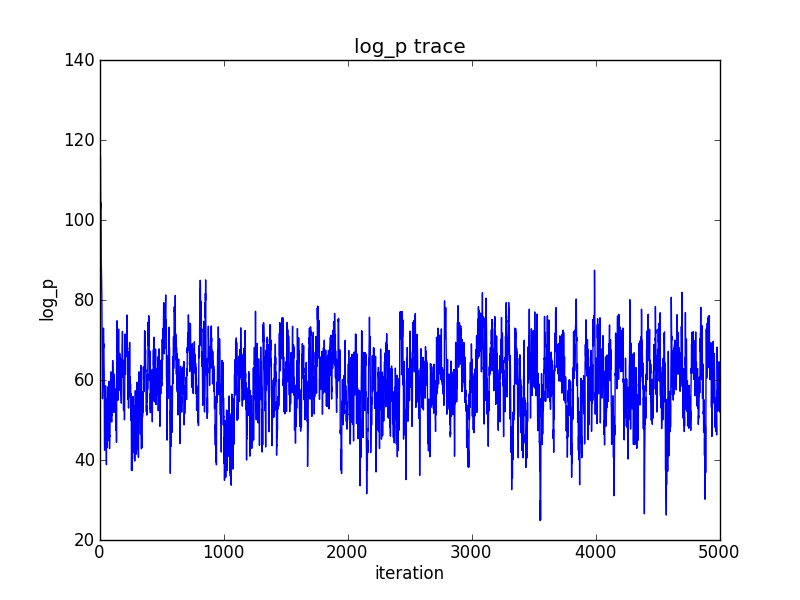
\includegraphics[width=.45\linewidth,height=0.3\textheight]{/Users/glareprotector/prostate_git/glare/tex_files/sections/simulate_data_points_infer_Bs/files/fixing_abc_log_p_trace.png}}
\end{subfigure}
\begin{subfigure}{
  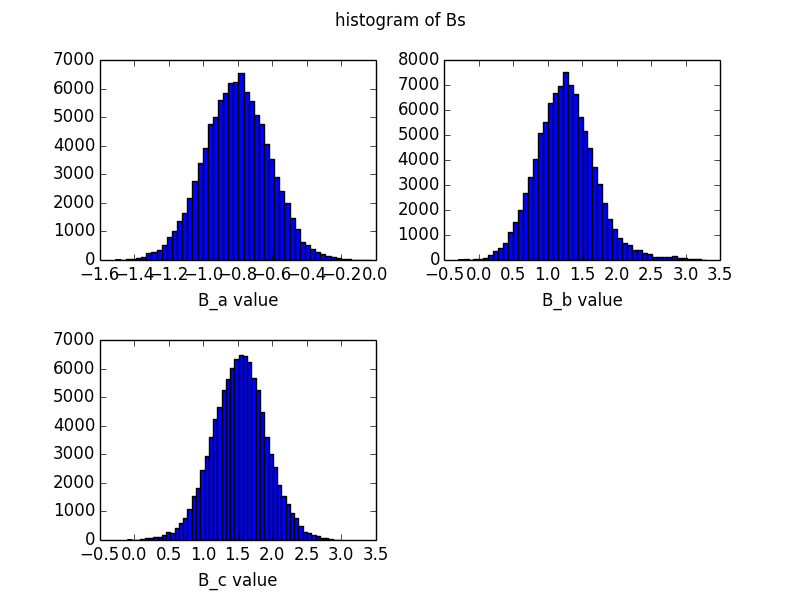
\includegraphics[width=.45\linewidth,height=0.3\textheight]{/Users/glareprotector/prostate_git/glare/tex_files/sections/simulate_data_points_infer_Bs/files/fixing_abc_Bs_histogram.png}}
\end{subfigure}
\begin{subfigure}{
  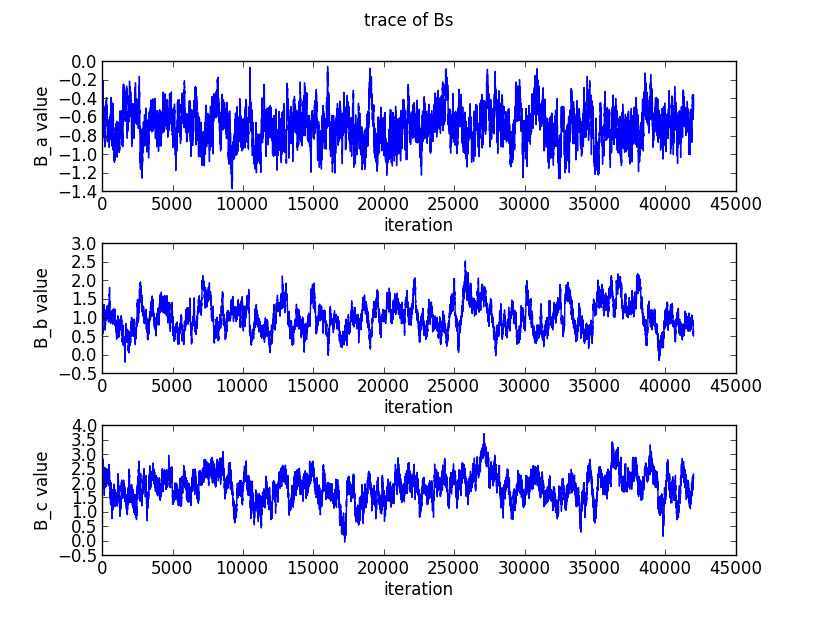
\includegraphics[width=.45\linewidth,height=0.3\textheight]{/Users/glareprotector/prostate_git/glare/tex_files/sections/simulate_data_points_infer_Bs/files/fixing_abc_Bs_trace.png}}
\end{subfigure}
\caption{Plots for when simulating $a,b,c$}
\end{figure}

\subsection{Simulating data points $g^*(t)$}
In the second scenario, we fix the $\phi^a,\phi^b,\phi^c$ and $B_a,B_b,B_c$ as before.  However, we do not simulate $a,b,c$ directly.  Rather, we picked a set of times $t_1 \ldots t_m$, and for each of the 15 patients, simulated $g_i^*(t_j)$ according to the model.  We set $\phi^{noise} = 0.1$.  That is, we first simulate $a_i, b_i, c_i$ and once those are determined, simulate $g_i^*(t_j)$ for each time point $t_j$.  To perform inference of $B_a, B_b, B_c$, we once again assume we know all noise parameters $\phi^a,\phi^b,\phi^c,\phi^{noise}$, and perform sampling to get the distribution of $P(B_a|\{g_i^*(t_j)\},\phi^a,\phi^b,\phi^c,\phi^{noise},X_i)$.

\begin{figure}
\centering
\begin{subfigure}{
  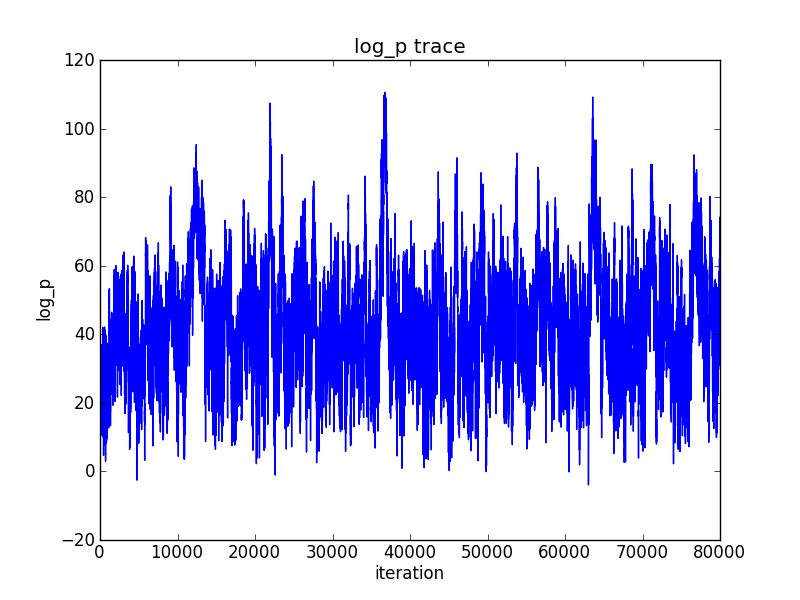
\includegraphics[width=.45\linewidth,height=0.3\textheight]{/Users/glareprotector/prostate_git/glare/tex_files/sections/simulate_data_points_infer_Bs/files/cmatters_log_p_trace.png}}
\end{subfigure}
\begin{subfigure}{
  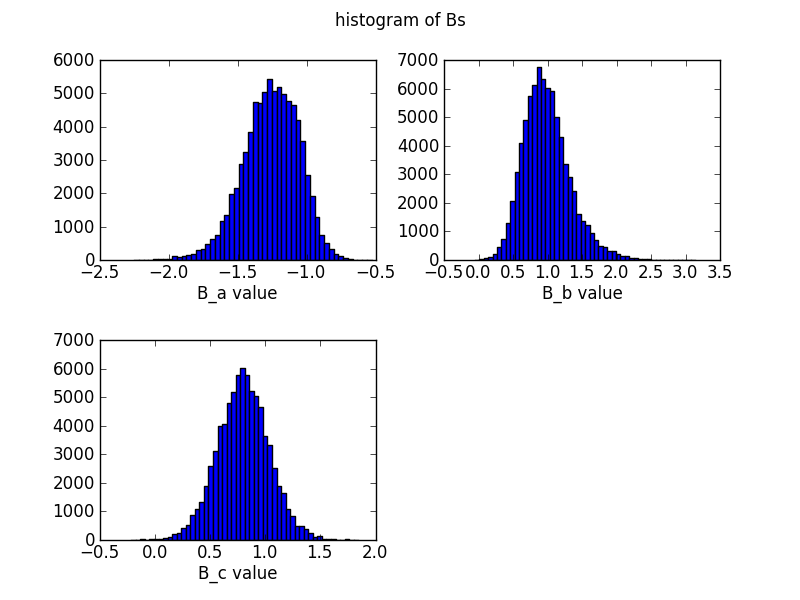
\includegraphics[width=.45\linewidth,height=0.3\textheight]{/Users/glareprotector/prostate_git/glare/tex_files/sections/simulate_data_points_infer_Bs/files/cmatters_Bs_histogram.png}}
\end{subfigure}
\begin{subfigure}{
  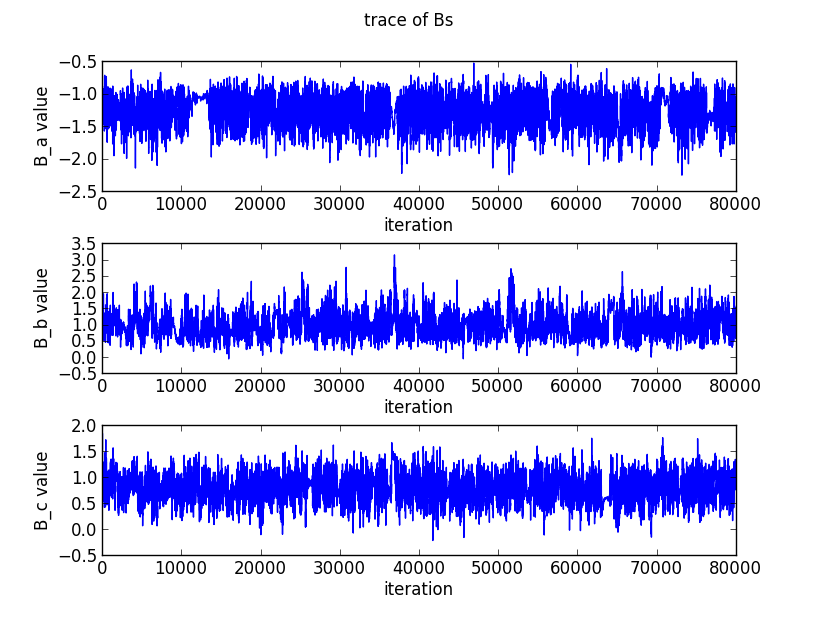
\includegraphics[width=.45\linewidth,height=0.3\textheight]{/Users/glareprotector/prostate_git/glare/tex_files/sections/simulate_data_points_infer_Bs/files/cmatters_Bs_trace.png}}
\end{subfigure}
\caption{Plots for when simulating $a,b,c$}
\end{figure}

